\documentclass[20pt]{article}

\usepackage{geometry}
\usepackage{titlesec}
\usepackage{amsmath}
\usepackage{amssymb}
\usepackage[T1]{fontenc}
\usepackage{times}
\usepackage{tipa}
\usepackage{covington}
\usepackage{tikz}
\usepackage{tikz-qtree}

\setlength\parindent{0pt}
\newcommand{\ipa}[1]{\textipa{#1}}
\newcommand{\broad}[1]{/\ipa{#1}/}
\newcommand{\narrow}[1]{[ \ipa{#1} ]}
\newcommand{\english}[1]{$<$#1$>$}
\newcommand{\sk}[0]{{\kern 0.05em}}
\newcommand{\mk}[0]{{\kern 0.1em}}
\newcommand{\smallcapi}[0]{\sk\textsci\sk}
\newcommand{\openo}[0]{\sk O}
\newcommand{\feature}[1]{\ensuremath{\left[ \text{#1} \right]}}
\newcommand{\treeScale}[0]{0.8}
\newcommand{\rolesOpacity}[0]{0.7}
\newcommand{\rolesOne}[0]{$<$$\theta$$>$}
\newcommand{\rolesTwo}[0]{$<$$\theta$,$\theta$$>$}
\newcommand{\rolesThree}[0]{$<$$\theta$,$\theta$,$\theta$$>$}
\newcommand{\constituent}[2]{$[_{\text{#1}}$ #2$]$}
\definecolor{darkgreen}{HTML}{006400}

\titlespacing*{\section}{0pt}{0.7\baselineskip}{0.7\baselineskip}
\titleformat*{\section}{\large\bfseries}

\begin{document}

\Large\textbf{Problem Set 8} \\
\normalsize
Alice McKean \\
\today

\section{Tree Structures}

\begin{tikzpicture}[scale=\treeScale, transform shape]
  \tikzset{every tree node/.style={align=center,anchor=north}}
  \Tree
  [.CP
    \node(WH-1-1){DP\\Who};
    [.C'
      \node(C-1-1){C\\\feature{Q}\feature{WH}\\would};
      [.TP
        \node(DP-1-1){DP\\you};
        [.T'
          \node(T-1-1){T\\$t$};
          [.VP
            \node(DP-1-2){$t$};
            [.V'
              V\\like
              [.CP
                \node(DP-2-1){$t$};
                [.C'
                  C\\\feature{WH}\\$\emptyset$
                  [.TP
                    \node(DP-2-2){DP\\\feature{PRO}};
                    [.T'
                      T\\to
                      [.VP
                        \node(DP-2-3){$t$};
                        [.V'
                          [.V'
                            V\\go
                            [.PP
                              P\\to
                              [.DP
                                D\\the
                                NP\\concert
                              ]
                            ]
                          ]
                          [.PP
                            P\\with
                            \node(DP-2-4){$t$};
                          ]
                        ]
                      ]
                    ]
                  ]
                ]
              ]
            ]
          ]
        ]
      ]
    ]
  ]
  \draw[->] (DP-2-3) to[bend left] (DP-2-2);
  \draw[->] (DP-2-4) to[out=-90,in=0] (10, -17.5) to[out=180,in=-90] (DP-2-1);
  \draw[->] (DP-2-1) to[bend left] (WH-1-1);
  \draw[->] (T-1-1) to[bend left] (C-1-1);
  \draw[->] (DP-1-2) to[bend left] (DP-1-1);
\end{tikzpicture} \\

\begin{tikzpicture}[scale=\treeScale, transform shape]
  \tikzset{every tree node/.style={align=center,anchor=north}}
  \Tree
  [.CP
    \node(C-1-1){C\\\feature{Q}\\Does};
    [.TP
      [.DP
        D\\\feature{PROP}
        \node(DP-1-1){NP\\Dorthy};
      ]
      [.T'
        \node(T-1-1){T\\$t$};
        [.VP
          \node(DP-1-2){$t$};
          [.V'
            V\\think
            [.CP
              C\\that
              [.TP
                [.DP
                  D\\\feature{PROP}
                  \node(DP-2-1){NP\\Edgar};
                ]
                [.T'
                  T\\will
                  [.VP
                    \node(DP-2-2){$t$};
                    [.V'
                      V\\convince
                      [.TP
                        [.DP
                          D\\the
                          \node(DP-3-1){NP\\children};
                        ]
                        [.T'
                          T\\to
                          [.VP
                            \node(DP-3-2){$t$};
                            VP\\participate
                          ]
                        ]
                      ]
                    ]
                  ]
                ]
              ]
            ]
          ]
        ]
      ]
    ]
  ]
  \draw[->] (T-1-1) to[out=-90,in=0] (0.7, -6) to[out=180,in=-90] (C-1-1);
  \draw[->] (DP-1-2) to[bend left] (DP-1-1);
  \draw[->] (DP-2-2) to[bend left] (DP-2-1);
  \draw[->] (DP-3-2) to[bend left] (DP-3-1);
\end{tikzpicture} \\

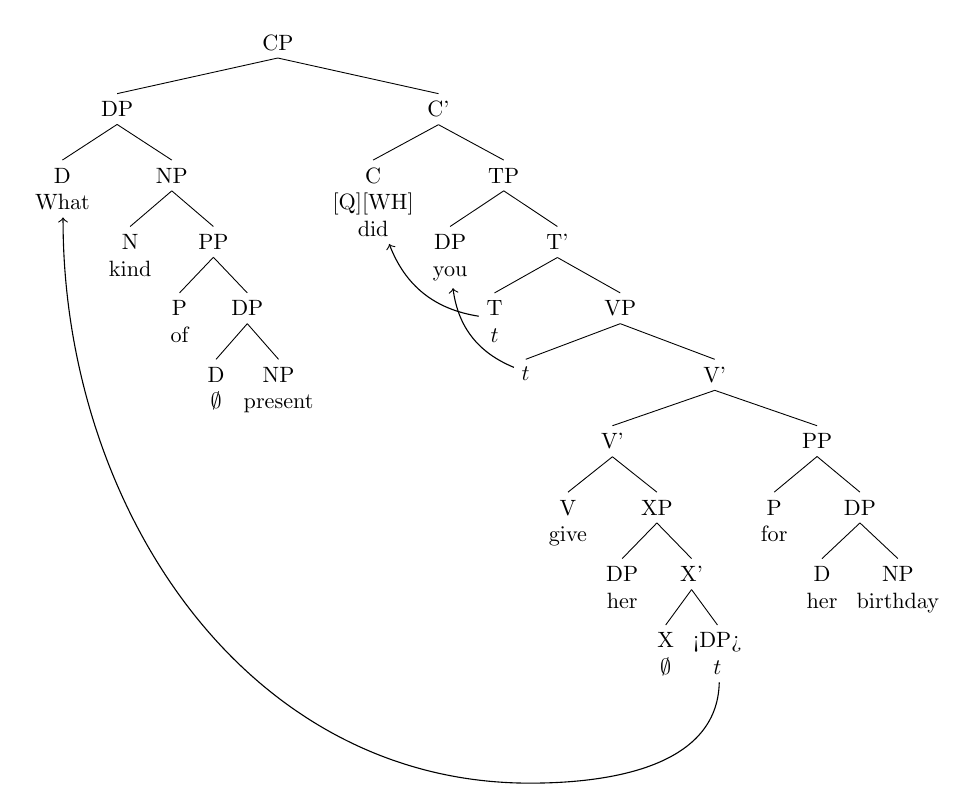
\begin{tikzpicture}[scale=\treeScale, transform shape]
  \tikzset{every tree node/.style={align=center,anchor=north}}
  \Tree
  [.CP
    [.DP
      \node(WH-1){D\\What};
      [.NP
        N\\kind
        [.PP
          P\\of
          [.DP
            D\\$\emptyset$
            NP\\present
          ]
        ]
      ]
    ]
    [.C'
      \node(Q-1){C\\\feature{Q}\feature{WH}\\did};
      [.TP
        \node(DP-1-1){DP\\you};
        [.T'
          \node(T-1){T\\$t$};
          [.VP
            \node(DP-1-2){$t$};
            [.V'
              [.V'
                V\\give
                [.XP
                  DP\\her
                  [.X'
                    X\\$\emptyset$
                    \node(WH-2){<DP>\\$t$};
                  ]
                ]
              ]
              [.PP
                P\\for
                [.DP
                  D\\her
                  NP\\birthday
                ]
              ]
            ]
          ]
        ]
      ]
    ]
  ]
  \draw[->] (DP-1-2) to[bend left] (DP-1-1);
  \draw[->] (T-1) to[bend left] (Q-1);
  \draw[->] (WH-2) to[out=-90,in=0] (4, -12) to[out=180,in=-90] (WH-1);
\end{tikzpicture} \\

\begin{tikzpicture}[scale=\treeScale, transform shape]
  \tikzset{every tree node/.style={align=center,anchor=north}}
  \Tree
  [.TP
    [.DP
      [.DP
        D\\\feature{PROP}
        NP\\George
      ]
      [.D'
        D\\-s
        \node(DP-1-1){NP\\Aunt};
      ]
    ]
    [.T'
      T\\was
      [.VP
        \node(DP-1-2){<DP>\\$t$};
        [.V'
          V\\asking
          [.CP
            [.AP
              DegP\\how
              \node(WH-1){AP\\tall};
            ]
            [.C'
              C\\\feature{WH}
              [.TP
                \node(DP-2-1){DP\\he};
                [.T'
                  T\\had
                  [.VP
                    \node(DP-2-2){$t$};
                    [.V'
                      [.V'
                        V\\grown
                        \node(WH-2){<AP>\\$t$};
                      ]
                      [.PP
                        P\\over
                        [.DP
                          D\\the
                          NP\\summer
                        ]
                      ]
                    ]
                  ]
                ]
              ]
            ]
          ]
        ]
      ]
    ]
  ]
  \draw[->] (DP-1-2) to[bend left] (DP-1-1);
  \draw[->] (DP-2-2) to[bend left] (DP-2-1);
  \draw[->] (WH-2) to[out=-90,in=0] (8, -14) to[out=180,in=-90] (WH-1);
\end{tikzpicture} \\

\begin{tikzpicture}[scale=\treeScale, transform shape]
  \tikzset{every tree node/.style={align=center,anchor=north}}
  \Tree
  [.TP
    [.DP
      D\\The
      \node(DP-1-1){NP\\critic};
    ]
    [.T'
      T\\\feature{PAST}
      [.VP
        \node(DP-1-2){$t$};
        [.V'
          V\\wondered
          [.CP
            \node(WH-2-1){DP\\what};
            [.C'
              C\\\feature{WH}
              [.TP
                \node(DP-2-1){DP\\\feature{PRO}};
                [.T'
                  T\\to
                  [.VP
                    \node(DP-2-2){$t$};
                    [.V'
                      [.V'
                        V\\say
                        \node(WH-2-2){$t$};
                      ]
                      [.PP
                        P\\about
                        [.DP
                          D\\the
                          NP\\performances
                        ]
                      ]
                    ]
                  ]
                ]
              ]
            ]
          ]
        ]
      ]
    ]
  ]
  \draw[->] (DP-1-2) to[bend left] (DP-1-1);
  \draw[->] (DP-2-2) to[bend left] (DP-2-1);
  \draw[->] (WH-2-2) to[out=-90,in=0] (7, -13) to[out=180,in=-90] (WH-2-1);
\end{tikzpicture} \\

\begin{tikzpicture}[scale=\treeScale, transform shape]
  \tikzset{every tree node/.style={align=center,anchor=north}}
  \Tree
  [.TP
    [.DP
      D\\\feature{PROP}
      \node(DP-1-1){NP\\Maurice};
    ]
    [.T'
      T\\\feature{PRES}
      [.VP
        \node(DP-1-2){<DP>\\$t$};
        [.V'
          V\\seems
          [.CP
            C\\$\emptyset$
            [.TP
              \node(DP-2-1){DP\\\feature{PRO}};
              [.T'
                T\\to
                [.VP
                  \node(DP-2-2){$t$};
                  [.V'
                    V\\want
                    [.TP
                      [.DP
                        D\\the
                        \node(DP-3-1){NP\\students};
                      ]
                      [.T'
                        T\\to
                        [.VP
                          \node(DP-3-2){$t$};
                          [.V'
                            [.V'
                              V\\work
                              [.DP
                                D\\$\emptyset$
                                NP\\together
                              ]
                            ]
                            [.PP
                              P\\on
                              [.DP
                                D\\the
                                NP\\assignment
                              ]
                            ]
                          ]
                        ]
                      ]
                    ]
                  ]
                ]
              ]
            ]
          ]
        ]
      ]
    ]
  ]
  \draw[->] (DP-1-2) to[bend left] (DP-1-1);
  \draw[->] (DP-2-2) to[bend left] (DP-2-1);
  \draw[->] (DP-3-2) to[bend left] (DP-3-1);
\end{tikzpicture}
\section{Binding Theory}
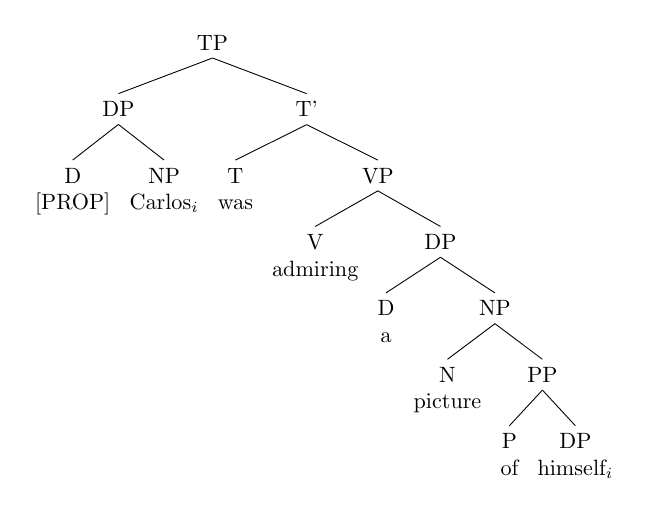
\begin{tikzpicture}[scale=\treeScale, transform shape]
  \tikzset{every tree node/.style={align=center,anchor=north}}
  \Tree
  [.TP
    [.DP
      D\\\feature{PROP}
      NP\\Carlos$_i$
    ]
    [.T'
      T\\was
      [.VP
        V\\admiring
        [.DP
          D\\a
          [.NP
            N\\picture
            [.PP
              P\\of
              DP\\himself$_i$
            ]
          ]
        ]
      ]
    ]
  ]
\end{tikzpicture} \\
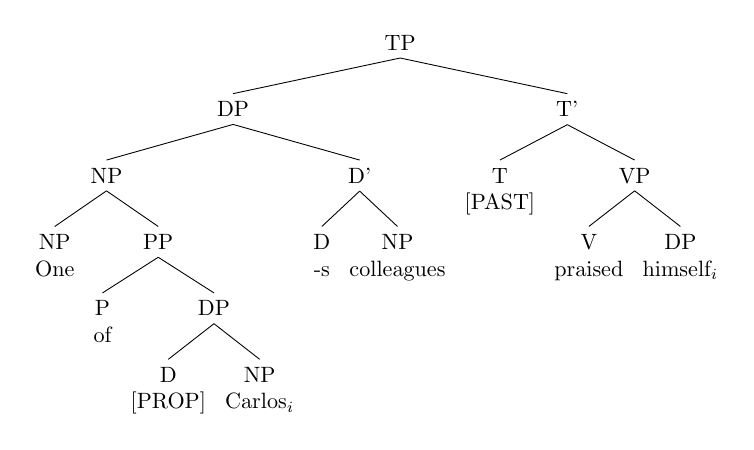
\begin{tikzpicture}[scale=\treeScale, transform shape]
  \tikzset{every tree node/.style={align=center,anchor=north}}
  \Tree
  [.TP
    [.DP
      [.NP
        NP\\One
        [.PP
          P\\of
          [.DP
            D\\\feature{PROP}
            NP\\Carlos$_i$
          ]
        ]
      ]
      [.D'
        D\\-s
        NP\\colleagues
      ]
    ]
    [.T'
      T\\\feature{PAST}
      [.VP
        V\\praised
        DP\\himself$_i$
      ]
    ]
  ]
\end{tikzpicture} \\

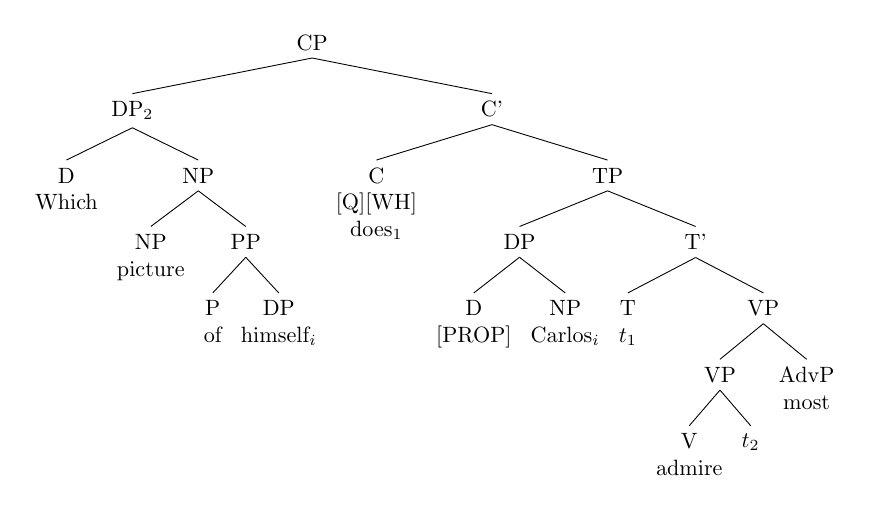
\begin{tikzpicture}[scale=\treeScale, transform shape]
  \tikzset{every tree node/.style={align=center,anchor=north}}
  \Tree
  [.CP
    [.DP$_2$
      D\\Which
      [.NP
        NP\\picture
        [.PP
          P\\of
          DP\\himself$_i$
        ]
      ]
    ]
    [.C'
      C\\\feature{Q}\feature{WH}\\does$_1$
      [.TP
        [.DP
          D\\\feature{PROP}
          NP\\Carlos$_i$
        ]
        [.T'
          T\\$t_1$
          [.VP
            [.VP
              V\\admire
              $t_2$
            ]
            AdvP\\most
          ]
        ]
      ]
    ]
  ]
\end{tikzpicture} \\

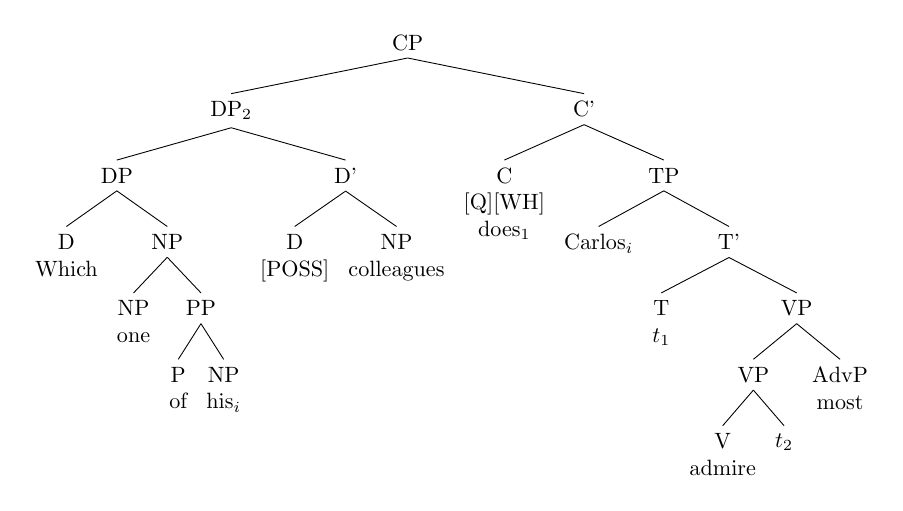
\begin{tikzpicture}[scale=\treeScale, transform shape]
  \tikzset{every tree node/.style={align=center,anchor=north}}
  \Tree
  [.CP
    [.DP$_2$
      [.DP
        D\\Which
        [.NP
          NP\\one
          [.PP
            P\\of
            NP\\his$_i$
          ]
        ]
      ]
      [.D'
        D\\\feature{POSS}
        NP\\colleagues
      ]
    ]
    [.C'
      C\\\feature{Q}\feature{WH}\\does$_1$
      [.TP
        Carlos$_i$
        [.T'
          T\\$t_1$
          [.VP
            [.VP
              V\\admire
              $t_2$
            ]
            AdvP\\most
          ]
        ]
      ]
    ]
  ]
\end{tikzpicture} \\

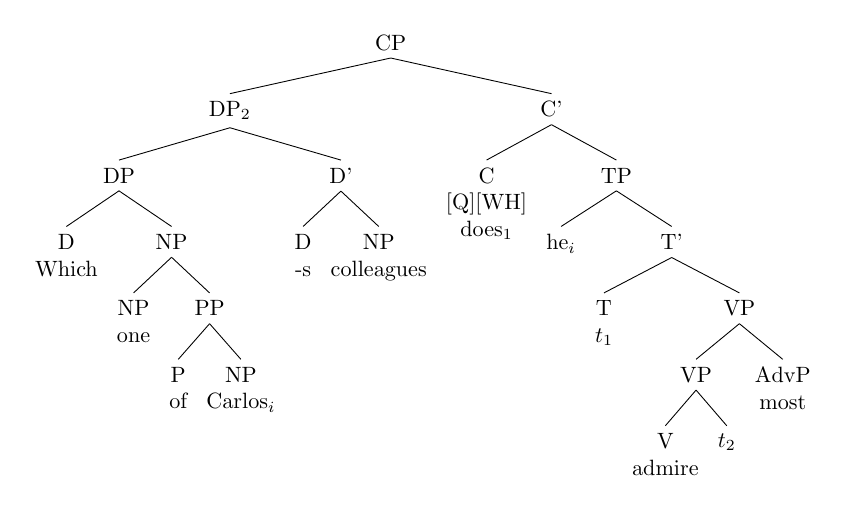
\begin{tikzpicture}[scale=\treeScale, transform shape]
  \tikzset{every tree node/.style={align=center,anchor=north}}
  \Tree
  [.CP
    [.DP$_2$
      [.DP
        D\\Which
        [.NP
          NP\\one
          [.PP
            P\\of
            NP\\Carlos$_i$
          ]
        ]
      ]
      [.D'
        D\\-s
        NP\\colleagues
      ]
    ]
    [.C'
      C\\\feature{Q}\feature{WH}\\does$_1$
      [.TP
        he$_i$
        [.T'
          T\\$t_1$
          [.VP
            [.VP
              V\\admire
              $t_2$
            ]
            AdvP\\most
          ]
        ]
      ]
    ]
  ]
\end{tikzpicture}
\end{document}

